\documentclass[12pt]{article}
%\usepackage[a4paper,left=2cm,right=2cm,top=2cm,bottom=2cm]{geometry}
\usepackage{graphicx}
\usepackage[utf8]{inputenc}
\usepackage{float}
\usepackage{caption}
\usepackage{amsmath}
\usepackage[backend=biber]{biblatex}
\usepackage{amssymb}
\usepackage{caption}
\bibliography{literature.bib}
\title{Machine Learning: Final project bomberchamp}
\date{today}
\begin{document}





\section{Introduction}
% Introduction
% we implemented a rainbow dqn

\subsection{Reinforcement Learning}
In reinforcement learning, sequential decision making problems need to be solved by an agent. The agent is provided with some input state and then needs to choose an action. Input state and chosen action are used to create a subsequent state and a reward signal for the agent. By maximizing the reward signals the agent develops a policy for acting in the environment and thus gets better in solving the given problem. Finding the optimal policy is the goal of reinforcement learning.
Hereby the environment is fully characterized by the state. \\
Time is discrete in reinforcement learning. Therefore the consecutive states form a chain.
Nevertheless transitions from one state to its subsequent state are not dependent on history, they only depend on the current state. This is called the Markov assumption. \\
For finding the optimal policy the state value function $V_\pi(s)$ can be used. It is defined as the expected reward of a policy $\pi$ that can be reached by starting at the state s
\begin{equation}
V_\pi=\mathbb{E}\left[R\right].
\end{equation}
The expected reward $R$ for a given state s is defined as the sum of the current reward and the discounted future rewards
\begin{equation}
R=\sum^\infty_{t=0}\,\gamma^t\,R_t \textrm{ for } s=s_0.
\end{equation}
$\gamma\:\epsilon\left[0,1\right]$ is the discount factor.\\
The optimal policy $\pi^*$ maximizes the state-value function.
% Reinforcement Learning basics a
\subsection{Neural Networks}
% basics j

\section{DQN}
%!TEX root = ./bomberchamp.tex
\subsection{Q-learning\anna}
In Q-learning \cite{DBLP:journals/corr/HasseltGS15} instead of the state-values, Q-values are being used. They are defined as the current reward depending on the chosen action and the discounted future rewards under the premise of always using the policy $\pi$ for further decision making after the initial action choice:
\begin{equation}
Q_\pi(s,a)=\mathbb{E}\left[R\right]|_{a,s,\pi}.
\end{equation} 
The best policy is then determined by maximizing $Q_\pi$ over the actions in every step.
%TODO why is this better than the state value function??
Usually it is not possible to learn every action for every state explicitly because the problems are often to extensive. Therefore the Q-values get approximated by a parametrized function $Q(s,a;\theta_t)$ with $\theta_t$ being the parameters. The Q-function is then updated towards the target value
\begin{equation}\label{eq:Q-target}Y_{t}^{\mathrm{Q}} \equiv R_{t+1}+\gamma \max _{a} Q\left(s_{t+1}, a ; \theta_{t}\right)
\end{equation}
after each action via:
\begin{equation}
\theta_{t+1}=\theta_{t}+\alpha\left(Y_{t}^{\mathrm{Q}}-Q\left(s_{t}, a; \theta_{t}\right)\right) \nabla_{\theta_{t}} Q\left(s_{t}, a ; \theta_{t}\right).
\end{equation}
This makes it an off-policy algorithm, as the optimal $Q$-value: $Q^*$ is approximated by $Q$ directly (regardless of the followed policy) in contrast to for example SARSA. The policy is still important as it determines, which state-action pairs are used to update the model \cite{Sutton:1998:IRL:551283}. 
Q-learning is also a model free approach, as it doesn't make a model of the environment but instead directly estimates $Q^*$.\\
%In our case with bomberman, the problem is fully observable, meaning that the agent knows the entire state of the environment at every step of the game.
\subsection{Q-Networks\anna}
For some reinforcement learning problems, the simplest implementation of the Q-learning algorithm, a table is perfectly sufficient to find a good policy.
If we consider more complicated problems with bigger inputs other methods are needed. For state of the art reinforcement learning, usually neural networks are being used.
They are especially convenient as they are trained from raw inputs, which makes handcrafted features redundant \cite{DBLP:journals/corr/MnihKSGAWR13}.
Neural Networks which are implemented to learn with the Q-algorithm are called Q-networks.
They are non linear function approximations for $Q(s,a;\theta_t)$.
To update the Q-network the loss function
\begin{equation}
L_{t}\left(\theta_{t}\right)=\mathbb{E}_{s, a \sim \rho(s,a)}\left[\left(Y_{t}^{\mathrm{Q}}-Q\left(s, a ; \theta_{t}\right)\right)^{2}\right]
\end{equation}
%TODO Erwartungswert großschreiben
is used, where $\rho(s, a)$ is a probability distribution over states and actions. To make this compatible with the Q-learning algorithm, the weights need to be updated at every step and the expectations exchanged with samples from the probability distribution $\rho(s,a)$.
\subsection{DQN\anna}
Deep Q-networks \cite{DBLP:journals/corr/MnihKSGAWR13} are multilayered neural networks which make use of the Q-learning algorithm. The two mayor improvements of the model are the use of two separate networks and an experience buffer.
The two networks are called online network and target network. The target network is used to calculate the targets $Y_{t}^{\mathrm{DQN}}$. It has the same structure as the online network but to make learning more stable, the weights of the target network $\theta_t^-$ stay constant for a longer time. 
They are being copied from the online network every $\tau$ steps.
The target is then calculated by:
\begin{equation}
Y_{t}^{\mathrm{DQN}} \equiv R_{t+1}+\gamma \max _{a} Q\left(s_{t+1}, a ; \theta_{t}^{-}\right).
\end{equation}
If only one network was used, an update of $Q(s,a)$ would often not only lead to a higher value of $Q(s_t,a_t)$ but also to higher expected Q-values $Q(s_{t+1},a)$ for all actions. If the target was also calculated by this network this could then lead to oscillations or divergence of the policy \cite{DBLP:journals/corr/MnihKSGAWR13}.
The additional improvement of DQN is experience replay. Without experience replay, only new experiences are used in training and discarded right afterwards.
Therefore important but rare experiences are almost immediately forgotten and the updates are not independent and identical distributed but strongly correlated. %TODO why is this bad?
To address this problem, an experience buffer is implemented. There the experiences are stored and then at training time sampled uniformly at random. Usually a simple FIFO algorithm is being used. But there are more sophisticated methods for this, one of those is discussed later.
% a

\section{Rainbow / DQN Extensions}
\subsection{Double DQN}
Q-learning  and DQN tend to learn overestimated action values. During the maximization over the action choices, values are rather over than underestimated.
This isn't necessarily a problem if they are uniformly overestimated or if interesting experiences are overestimated. However, in DQN overestimations differ for different actions and states. Combined with bootstrapping, this results in the propagation of wrong values and thus to worse policies \cite{DBLP:journals/corr/HasseltGS15}. To reduce those overestimations, the Double Q-learning algorithm \cite{DBLP:journals/corr/HasseltGS15} is used. 
The main idea of the Double Q-learning algorithm is to decouple value selection and evaluation.
DQN, with separate online and target networks provides an excellent framework for this decoupling:
The online network is used to select an action from the action choices via maximization whereas the target network evaluates the actions to generate the Q-values.
The resulting double DQN yields more accurate values and hence leads to better policies than DQN \cite{DBLP:journals/corr/HasseltGS15}.
Updating double DQNs is similar to updating DQNs when the target is rewritten as:
\begin{equation}\label{eq:DDQN-target}
Y_{t}^{\text { Double DQN }} \equiv R_{t+1}+\gamma Q\left(s_{t+1}, \underset{a}{\operatorname{argmax}} Q\left(s_{t+1}, a ; \theta_{t}\right); \theta_{t}^{-}\right).
\end{equation}
$\theta_{t}^{-}$ and $\theta_{t}$ are the weights of the target and online network respectively.
\subsection{Prioritized Experience Replay}
In standard experience replay, the agent is forced to pick experiences uniformly from all experiences in its memory. Therefore all experiences are sampled with the same frequency that they were originally encountered.
This is not necessarily good for the learning process, as some experiences might not hold any valuable information for the agent but occur very often while other rare situations could be crucial for learning. \\
This can be improved by prioritized experience replay \cite{DBLP:journals/corr/SchaulQAS15}. Here every experience in the buffer gets a priority according to its TD-error.
The TD-error measures the difference between the actual Q-value and the Target-Q-value, so if experiences with bigger TD-errors are provided with bigger priorities, experiences from which there still is a lot to learn are favoured.
The priority $p_i$ is determined from the TD-error $\delta_i$ according to:
\begin{equation}
p_{i}=\left|\delta_{i}\right|+\epsilon.
\end{equation}
Hereby $\epsilon\,>\,0$ denotes a small parameter to ensure, that every experience has a priority bigger than zero and thus can be picked for a sample batch.
New experiences are always added with maximum priority to the memory.
Problematic with this greedy approach is, that only experiences that are picked for learning get their priority updated. Therefore experiences with low initial priority might, because of the buffer memory structure be removed from memory before they could have been picked for learning. The buffer is also very sensitive to noise spikes \cite{DBLP:journals/corr/SchaulQAS15}. \\
To overcome this problems stochastic prioritization is used and $p_i$ adjusted according to:
\begin{equation}
P(i)=\frac{p_{i}^{\alpha}}{\sum_{k} p_{k}^{\alpha}}.
\end{equation}
Here $\alpha\,\epsilon\,[0,1]$ is another parameter which adjusts the amount of prioritization that is used. For $\alpha=0$ we get the uniform case (no prioritization), whereas $\alpha=1$ leads to greedy prioritization. \\
Stochastic prioritization introduces bias to our model. This needs to be considered for updating the model, because it could change the solution the model is converging to \cite{DBLP:journals/corr/SchaulQAS15}. To correct this, importance sampling weights (IS weights) are introduced: 
\begin{equation}
w_{i}=\left(\frac{1}{N} \cdot \frac{1}{P(i)}\right)^{\beta},
\end{equation}
with N being the replay buffer size and $\beta\,\epsilon\,[0,1]$ being a hyperparameter for  adjustment of the bias. 
For $\beta=1$ the bias gets fully compensated. This is most important at the end of the training process. Therefore $\beta$ starts at an initial value and is then being annealed during training. \\\\
An efficient data structure for the memory is crucial for good performance.
To guarantee this, we implemented a sum tree to store the data, where searching is of complexity $O(1)$ and updating of complexity $O(\log N)$.
A sum tree is a binary tree, in which the parent node values are the sum of the child node values. In our sum tree, the transition priorities were saved in the leave nodes. Therefore the root holds the total priority. An array was used to hold the associated data values to the priorities. For the purpose of sampling the total priority is divided into k priority ranges, with k being the number of experiences in one sample.
From each of these priority ranges one value is sampled uniformly and its corresponding leave node is searched. The data belonging to this priority is than used for the sample.

\subsection{Duelling networks}
The idea behind duelling networks \cite{DBLP:journals/corr/WangFL15} is, that for some states only the state-value function is important while for others the chosen action is crucial. \\
Consider a small toy problem: Our agent needs to catch coins which are falling down form above, he can either move right or left or wait to catch them. In some states there are no coins at all. In that state it is not important which action is chosen, whereas for other states its is.
\begin{figure}
\centering
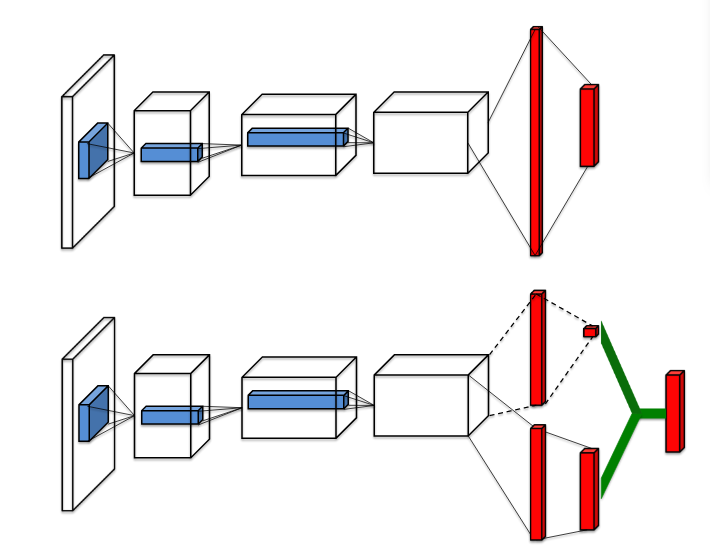
\includegraphics[scale=0.5]{./images/dueling.png}
\caption{Top: Standard Deep Q-network. Bottom: Dueling DQN with two separate streams \cite{DBLP:journals/corr/WangFL15}.}
\label{fig: dueling}
\end{figure}
To exploit this the neural network is split into two streams: 
the action and the state-value stream, as can be seen in figure \ref{fig: dueling}. The network is split after the convolutional layers. Therefore the two streams consist of linear layers. The benefit of this is, that it is possible to get separate estimations for state-value function and action-value function. Hereby the state-value $V(s ; \theta, \beta)$ is a scalar property while the action-vector $A(s, a ; \theta, \alpha)$ has the dimension of the quantity of possible action choices, in our case six. $\theta$ are the weights of the convolutional layers, while $\alpha$ and $\beta$ are the weights for the A- and the V- stream respectively. \\
For getting the Q-value A and V need to be recombined. It is not a good idea though to simply add them together:
\begin{equation}
Q(s, a ; \theta, \alpha, \beta)=V(s ; \theta, \beta)+A(s, a ; \theta, \alpha).
\end{equation}
In that case it would get impossible to retrieve V and A from Q uniquely. One could add a constant to A and subtract it from V without changing Q.
It is better to calculate Q by
\begin{equation}
Q(s, a ; \theta, \alpha, \beta)=V(s ; \theta, \beta)+ \left(A(s, a ; \theta, \alpha)-\frac{1}{|\mathcal{A}|} \sum_{a^{\prime}} A\left(s, a^{\prime} ; \theta, \alpha\right)\right),
\end{equation}
where A and V keep their identifiability and the optimization becomes more stable \cite{DBLP:journals/corr/WangFL15}.
\subsection{Noisy Networks}
So far we did use an $\epsilon$-greedy policy for exploration. Another technique which has been found to produce better result for many of the Atari games are Noisy Nets \cite{DBLP:journals/corr/FortunatoAPMOGM17}. They add parametric noise to the weights and thus aid exploration without the need to pick random actions as part of a policy (e.g. $\epsilon$-greedy). This is very convenient, because there is no need to tune additional hyper parameters as the reinforcement learning algorithm tunes the weights automatically.
Consider a neural network $y=f_{\theta_n}(x)$. Where $\theta_n$ are the noisy weights. A linear layer of a neural network can be written as: 
\begin{equation}
y = w x+b,
\end{equation}
whereas a noisy linear layer can be written as:
\begin{equation}
y =\left(\mu^{w}+\sigma^{w} \odot \varepsilon^{w}\right) x+\mu^{b}+\sigma^{b} \odot \varepsilon^{b}.
\end{equation}
Here $x$ is the input, $w$, and $\mu^{w}+\sigma^{w} \odot \varepsilon^{w}$ are the weights and $b$ and $\mu^{b}+\sigma^{b} \odot \varepsilon^{b}$ are the biases for linear and noisy linear layer respectively. All of the named parameters are trainable except for $\varepsilon^w$ and $\varepsilon^b$ which are noise random variables. We chose factorized gaussian noise for the distribution of the $\varepsilon$ parameters, as it reduces computation time for random number generation, which is important for single thread-agents such as ours \cite{DBLP:journals/corr/FortunatoAPMOGM17}. Here only one independent noise per input and another independent noise per output is needed, in contrast to independent Gaussian noise, where one independent noise per weight would be required.
We factorized $\varepsilon^w$ to $\varepsilon^w_{i,j}$.
The noise random variables can then be written as:
\begin{equation}
\begin{aligned} \varepsilon_{i, j}^{w} &=f\left(\varepsilon_{i}\right) f\left(\varepsilon_{j}\right) \\ \varepsilon_{j}^{b} &=f\left(\varepsilon_{j}\right) \end{aligned},
\end{equation}
where we used \begin{equation}
f(x)=\operatorname{sgn}(x) \sqrt{|x|}.
\end{equation}
The parameters $\mu_{i,j}$ were initialized as samples from a random uniform distribution $\left[-\frac{1}{\sqrt{p}},+\frac{1}{\sqrt{p}}\right]$ with $p$ being the number of inputs for the noisy linear layer. $\sigma_{i, j}$ were set as $\sigma_{i, j}=\frac{\sigma_{0}}{\sqrt{p}}$. \\
For the Noisy Networks implementation we replaced the Fully Dense layers of the state-value and action streams by Noisy layers. %TODO Loss changes?
\cite{DBLP:journals/corr/FortunatoAPMOGM17}
\subsection{Multi-Step Learning} % j
% 
%!TEX root = ../bomberchamp.tex
We are trying to learn the total discounted return
$$Q^{*}(x_t, a_t)=R(x_t, a_t)+\gamma R(x_{t+1}, a_{t+1})+\gamma^2 R(x_{t+2}, a_{t+2}) + ...$$

If we assume that we use the optimal policy for $t+1$ onward, we can substitute $\gamma R(x_{t+1}, a_{t+1})+\gamma^2 R(x_{t+2}, a_{t+2}) + ...$ with $Q^{*}(x_{t+1}, a*_{t+1}$.

Q-Learning takes the reward from a single step and adds the discounted value estimate of the greedy action at the next step.

$$\hat{Q}^{*}(x_t, a_t)=R(x_t, a_t)+\gamma \hat{Q}^{*}(x_{t+1}, a_{t+1})$$

For multi-step Q-Learning we take the n-step truncated return
$$R_{t}^{(n)} \equiv \sum_{k=0}^{n-1} \gamma_{t}^{(k)} R_{t+k+1}$$

to estimate the


\section{Other things}
\subsection{Augmented data}   %a
\vspace{1 cm}
\begin{minipage}{\textwidth}
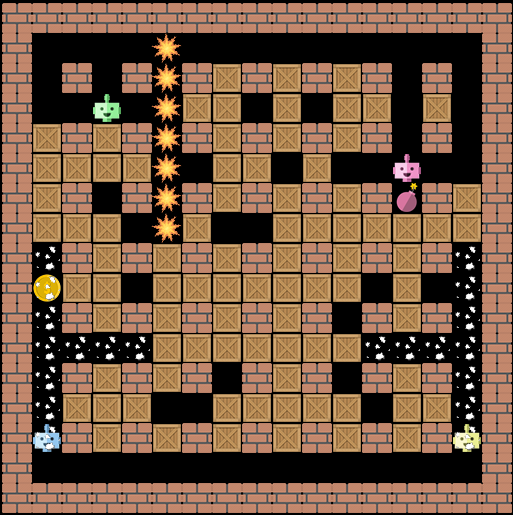
\includegraphics[scale=0.3]{./images/augmented_original.png}
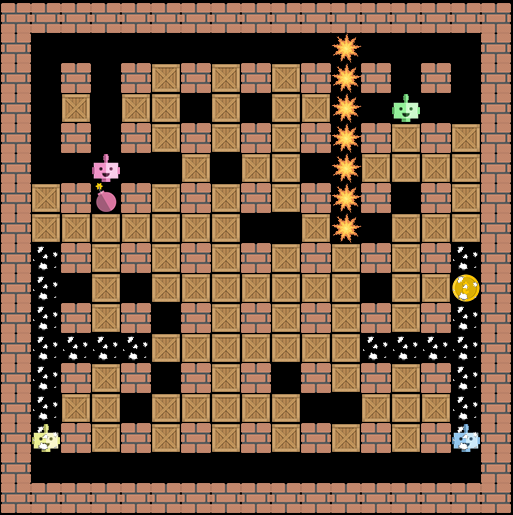
\includegraphics[scale=0.3]{./images/augmented_lr.png}
\end{minipage}
\begin{minipage}{\textwidth}
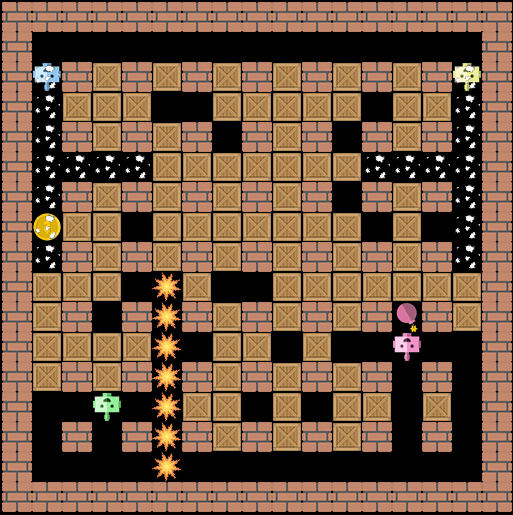
\includegraphics[scale=0.3]{./images/augmented_ud.png}
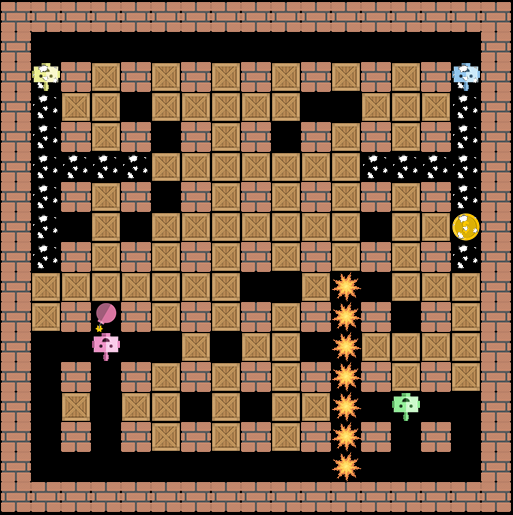
\includegraphics[scale=0.3]{./images/augmented_udlr.png}
\captionof{figure}{Data augmentation: \newline Upper left: original; Upper right: horizontal mirroring; \newline Lower left: vertical mirroring; Lower right: combined mirroring}
\label{fig:augmented}
\end{minipage}
\newline
\newline
\newline
\newline
As the inputs for our bomberchamp agent are symmetric, we wanted to use data augmentation to increase the number of samples for training and to make learning more symmetric.
From each original sample, three augmented samples were created. For augmentation, we had to mirror the environment and to change action choices accordingly. The augmented environment consisted of horizontal mirroring, vertical mirroring and a combination of both as seen in figure \ref{fig:augmented}.
For horizontal mirroring the agent choices left and right were exchanged, for vertical mirroring up and down and for the combination both were swapped. \newline
Data augmentation did not work as well as we expected, so it was not included in our final implementation (more details in the next section).
\subsection{Centring of agent} % j / a
\subsection{Invalid actions} % 
%!TEX root = ../bomberchamp.tex

We're only selecting from valid actions, since we found that otherwise the invalid actions can cause a lot of trouble. (essentially invalid actions are equal to WAIT, meaning that the rewards for different actions get mixed up)
Another solution would've been to penalize invalid actions and let the agent learn to avoid them, but since filtering out invalid action is really easy and fast, we use that.

\subsection{Auxilliary Reward Design}
%!TEX root = ../bomberchamp.tex

Auxilliary rewards:
For coin collection, 


For single player with coins in crates, interestingly it did learn to destroy the crates and collect the coins pretty well with a reward for destroying crates and no penalty for death. But there were a lot of games where the agent bombed itself in the beginning.
With a penalty for death, the agent learns to avoid death by choosing WAIT. Therefore we penalize this action and the agent learns to destroy the crates and collect coins, but when run too long, it learns to alternate UP-DOWN and RIGHT-LEFT to avoid death.

depending on the crate reward, the agent may ignore coins

In multi-player, without auxilliary rewards, the agent does not learn well.
With auxilliary rewards for crates and WAIT, the agent learns well.

\subsection{Minigame Collection} % j
\subsection{Self-Play} % j

\section{Observation}
\subsection{It does not work}
% nothing works
% solution: make it better
\subsection{Network scaling} % j
% different networks from minigame to full game
% lots of graphs

% our learning process


\section{Summary and Improvements}
% improvements: distributional DQN, train for 3 months

% improvement of game setup: j
% - make provided framework easy to use
% -- currently main.py, settings.py and possibly callbacks.py has to be changed for a simple switch between train and test mode
% -- separate rendering and environment, so that the environment can be called from e.g. a jupyter notebook
% -- provide main.py or python notebook 





\section{Model}



\section{Training process}


\subsection{Centring of the agent}
To simplify learning for our agent, it was centred on the board, so that it stays at a fixed position while the environment (coins, crates, other agents) move around it. This is very common in the Atari games on which most implementations of DQN agents are tested, including the Rainbow agent without distributional reinforcement learning from which we took most of our initial hyper parameters. Therefore we thought, a more similar setting would be beneficial to our agent. To implement this, the size of the board was increased to four times its original size and the agent placed in the middle of the new board.
\subsection{Self play}
%TODO how was it implemented etc
For training purposes a simple agent implementation that follows the rules of bomberman and plays reasonably well was provided.
To exploit this we wanted to first train our agent by classifying inputs generated with the simple agents. %TODO why didn't this work?
This is why we implemented a self play strategy. This was also useful, as we could then use google colab and train more than one agent at the same time while using the same neural network.



\printbibliography

\end{document}
